Интерферометр Фабри–Перо как спектральный прибор высокой разрешающей
силы находит широкое применение в лабораторной практике.
Он предназначен главным образом для исследования тонкой структуры
спектральных линий, а также является неотъемлемым элементом любого лазера,
 где выполняет роль оптического резонатора.

 \begin{wrapfigure}{r}{0.4\linewidth}
    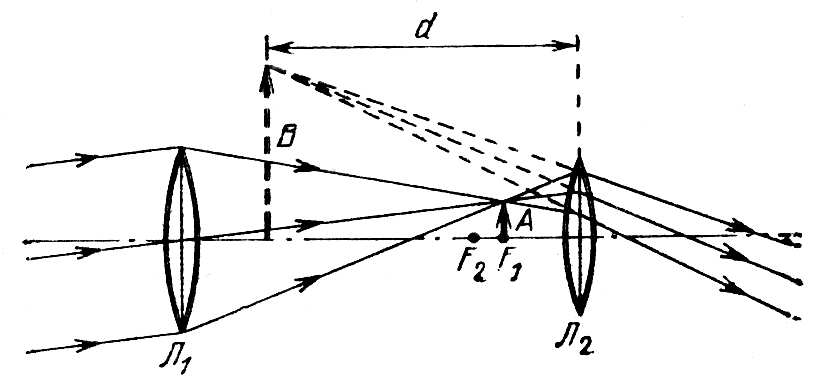
\includegraphics[width=\linewidth]{1.png}
    \caption{Интерферометр Фабри–Перо}
    \label{img::1}
 \end{wrapfigure}

\par Интерферометр Фабри–Перо состоит из двух стеклянных (или кварцевых) 
пластин $P_1$ и $P_2$ (рис. \ref{img::1}), внутренние плоские поверхности 
которых хорошо отполированы (с точностью до $10^{-2}\lambda$) и установлены
параллельно друг другу. На эти поверхности наносятся хорошо отражающие покрытия.
Наряду с металлическими покрытиями ($Ag$, $Al$), для которых
коэффициент отражения $r \simeq 0.9$, в настоящее время широко 
применяются диэлектрические многослойные интерференционные 
покрытия, для которых $r \simeq 0.99$ и даже выше. 
Наружные поверхности пластин обычно составляют небольшой угол 
с внутренними, чтобы световой блик, отражённый от наружных 
поверхностей, не мешал наблюдениям.

Интерферометр Фабри–Перо можно рассматривать как плоскопараллельную 
воздушную пластину, на которой происходят многократные отражения и 
интерференция световых лучей. 
Интерференционная картина, наблюдаемая в фокальной плоскости 
линзы $Л$, состоит из концентрических колец равного наклона. 
Для двух соседних лучей, распространяющихся между зеркалами 
интерферометра под углом $\theta$, разность хода определяется соотношением

\begin{equation}\label{eq::1}
  \Delta = 2L \cos{\theta},
\end{equation}
\noindent где $L$ ~---~ расстояние между зеркалами интерферометра. 
Равенство \eqref{eq::1} ~---~ частный случай известной формулы для плоскопараллельной пластины
с показателем преломления $n$: $\Delta = 2Ln \cos{\psi}$;
$\psi$ ~---~ угол преломления луча в пластине.

Пусть $r$ и $t$ ~---~ коэффициенты отражения и пропускания зеркал интерферометра (по интенсивности).
Если амплитуду падающей волны обозначить через $A_0$, то амплитуда 
первого луча, прошедшего через интерферометр, равна $A_0t$, 
второго $A_0tr$, третьего $A_0tr^2$ и т.~д.
В комплексном представлении амплитуды этих лучей составляют бесконечную геометрическую прогрессию
\begin{equation}\label{eq::2}
  A_0t, \: 
  A_0tr\e^{\iu k \Delta}, \: 
  A_0tr^2\e^{\iu 2k \Delta}, \:
  A_0tr^3\e^{\iu 3k \Delta}, \:
  \dots , 
\end{equation}
\noindent где $k = \frac{2\pi}{\lambda}$ ~---~ волновое число 
для света. Знаменатель прогрессии равен $r\e^{\iu k\Delta}$. 
В фокальной плоскости линзы происходит сложение всех лучей.
Результирующая амплитуда равна
\begin{equation}\label{eq::3}
  A = \frac{A_0t}{1 - re^{\iu k\Delta}}.
\end{equation}
Найдём интенсивность $I$ прошедшего света:
\begin{equation}\label{eq::4}
  I = AA^* = \frac{I_0t^2}{1 + r^2 - 2r\cos{k\Delta}},
\end{equation}
где $I_0 = A^2_0$ ~---~ интенсивность падающей волны. 
На рис. \ref{img::2} представлена зависимость отношения $\frac{I}{I_0}$ 
от порядка интерференции $\frac{\Delta}{\lambda}$ для разных
значений коэффициента отражения. Как видно из \eqref{eq::4}, 
максимумы этого распределения достигаются при целых значениях
$\frac{\Delta}{\lambda}$. При этом $I_{max} = I_0$, т.~е. 
интерферометр в этом случае является идеально прозрачной системой.
Разумеется, этот результат справедлив только в отсутствие поглощения света в зеркалах.
При достаточно больших значениях коэффициента отражения ($r \gtrsim 0.9$)
интерференционная картина состоит из узких светлых колец, 
разделённых широкими тёмными промежутками. Это является следствием
интерференции большого числа лучей (многолучевая интерференция).
При $r \lesssim 0.1$ наблюдается плавное чередование слабо выраженных 
максимумов и минимумов, характерное для интерференции двух лучей,
сильно различающихся по амплитуде.